\clearpage
\section{MODELAGEM VISUAL ATUALIZADA}

Esta seção apresenta a modelagem visual atualizada conforme a estrutura hierárquica macro definida, organizando as entidades desde o nível regulatório até a execução operacional.

% ================================================================
% DIAGRAMA 1: MODELO MACRO COMPLETO
% ================================================================

\subsection{Modelo Macro Institucional}

\begin{figure}[H]
    \centering
    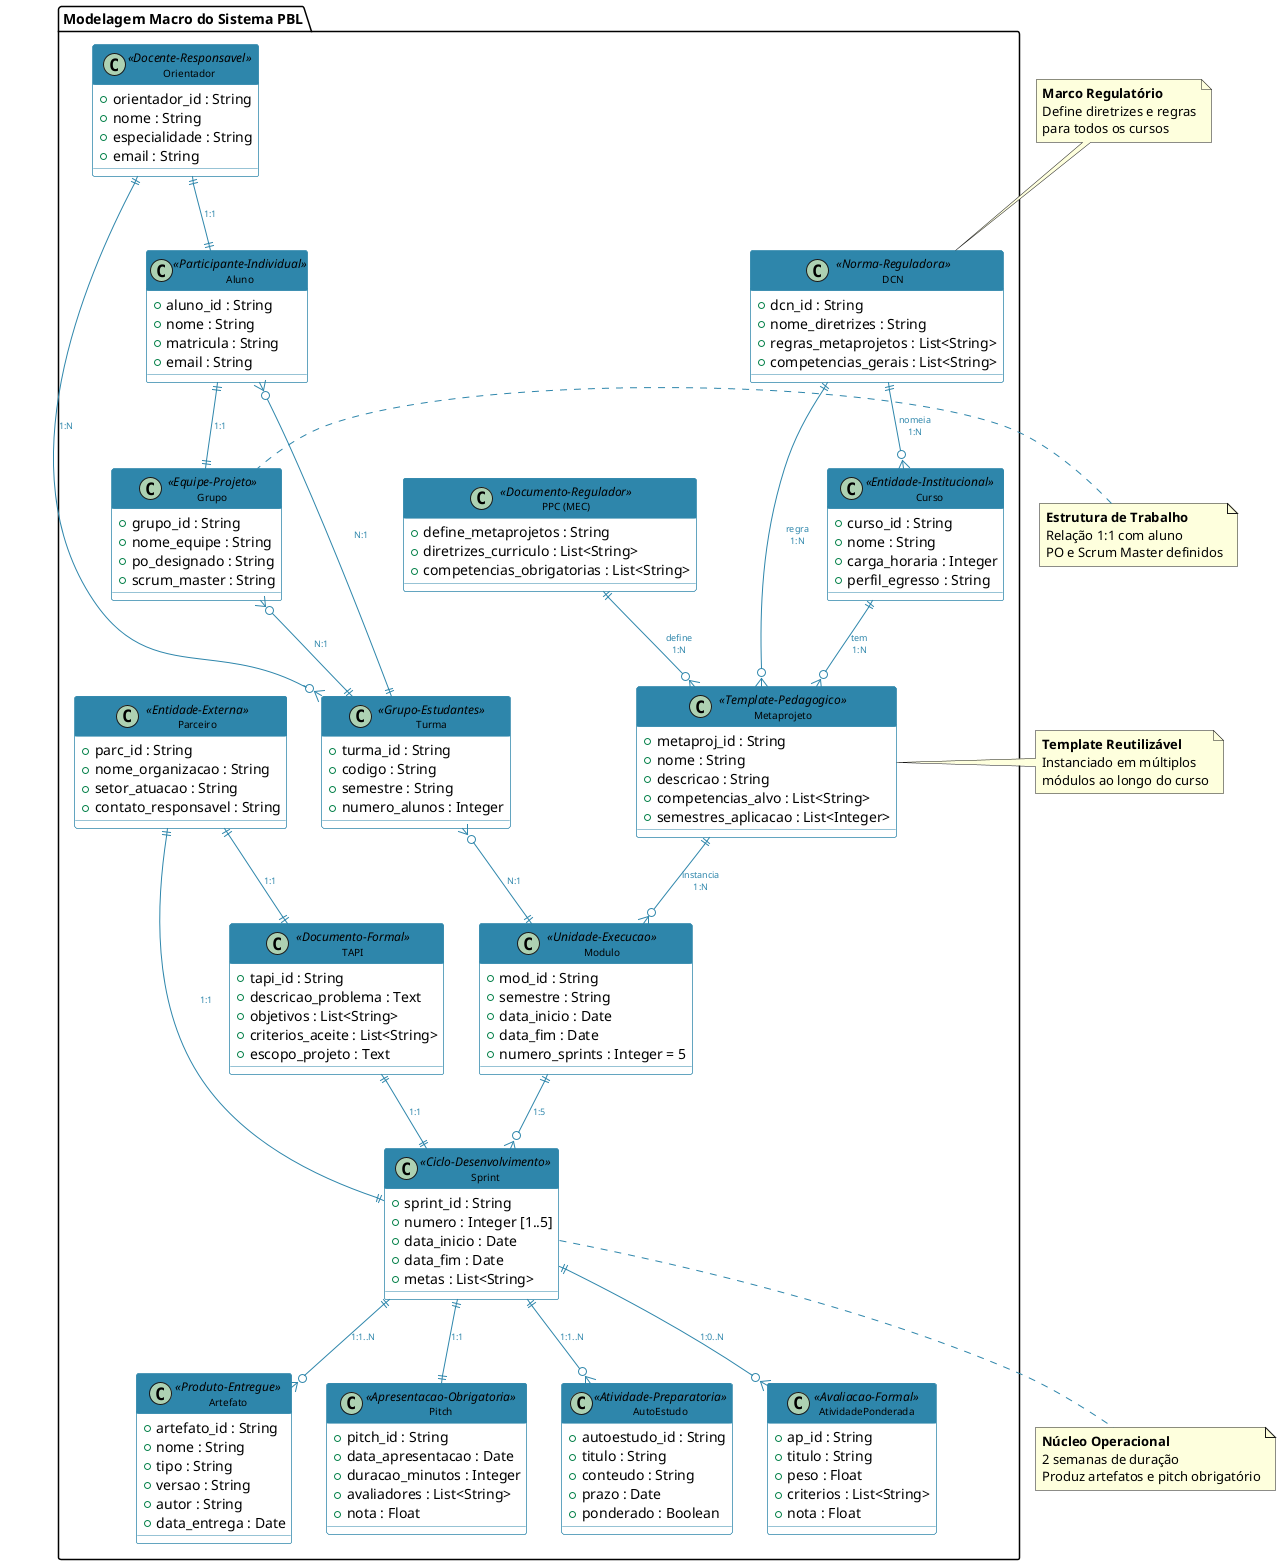
\includegraphics[width=0.95\textwidth]{plantuml/diagrama1_modelo_macro}
    \caption{Modelagem macro: hierarquia institucional completa (DCN → Curso → Metaprojeto → Módulo)}
    \label{fig:modelo_macro_completo}
\end{figure}

O modelo macro estabelece a hierarquia institucional completa: \textbf{DCN} normatiza \textbf{Cursos} e estabelece regras para \textbf{Metaprojetos}, \textbf{PPC (MEC)} define Metaprojetos, cada \textbf{Curso} tem múltiplos Metaprojetos que se instanciam em \textbf{Módulos} específicos. A relação \textbf{Parceiro-TAPI-Sprint} (1:1:1) contextualiza cada ciclo de desenvolvimento.

% ================================================================
% DIAGRAMA 2: ESTRUTURA OPERACIONAL
% ================================================================

\subsection{Estrutura Operacional do Módulo}

\begin{figure}[H]
    \centering
    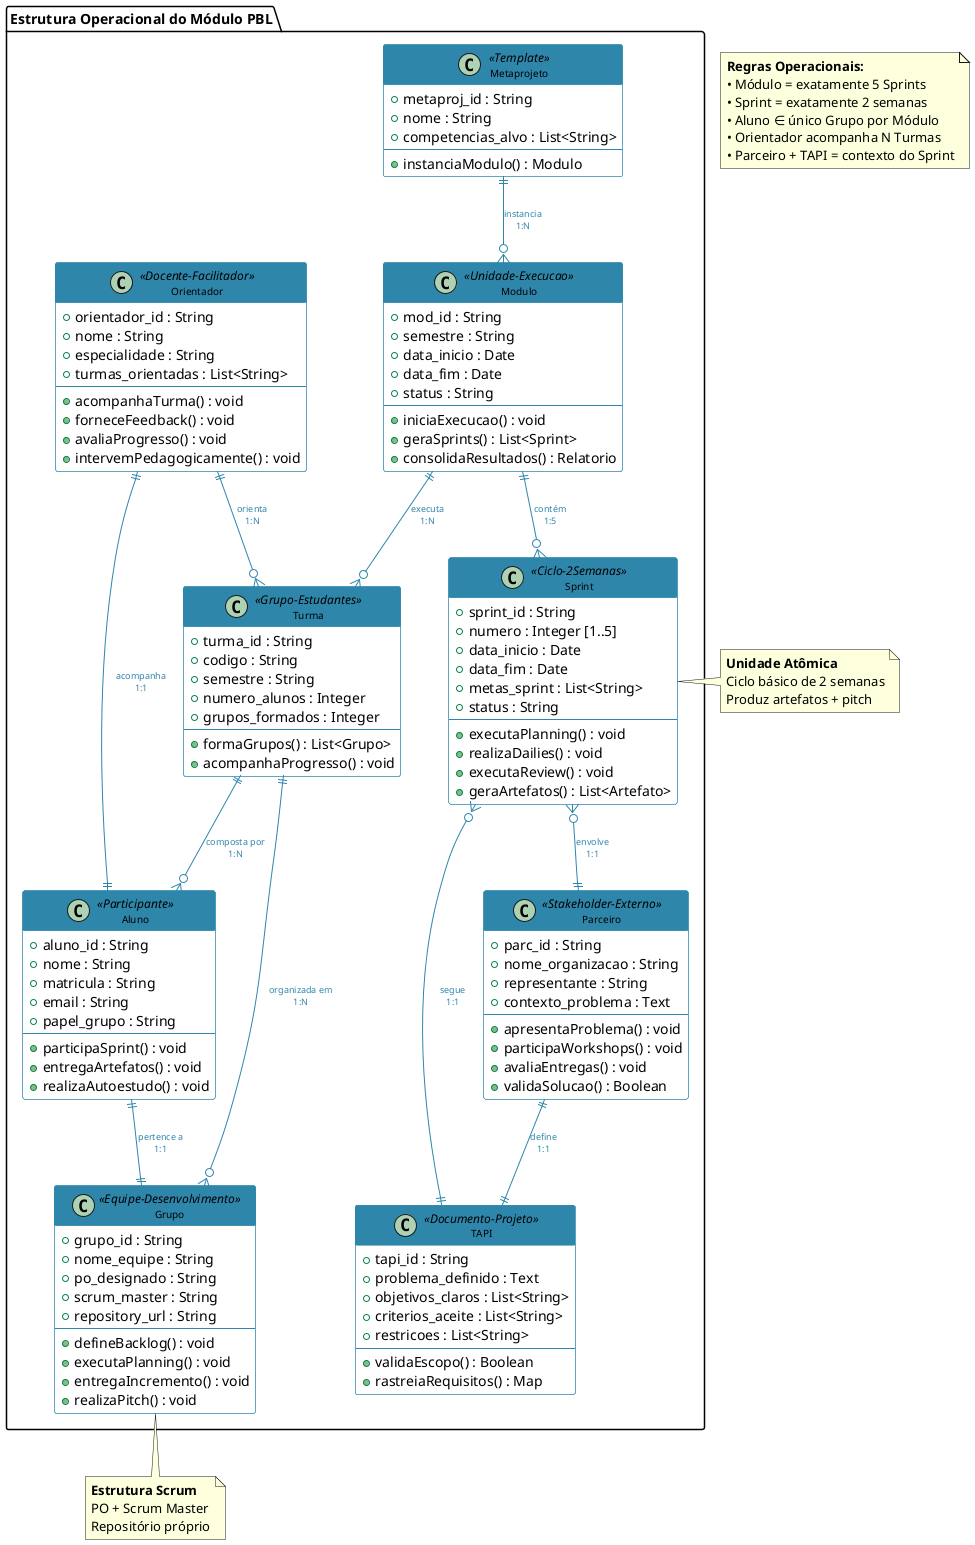
\includegraphics[width=0.9\textwidth]{plantuml/diagrama2_estrutura_operacional}
    \caption{Estrutura operacional: Módulo, Sprint, Turma, Aluno, Grupo e Orientador}
    \label{fig:estrutura_operacional}
\end{figure}

A estrutura operacional organiza a execução: \textbf{Módulo} contém exatamente 5 \textbf{Sprints} e múltiplas \textbf{Turmas}. Cada \textbf{Turma} compõe-se de \textbf{Alunos} organizados em \textbf{Grupos} (relação 1:1). \textbf{Orientador} acompanha N Turmas com relacionamento específico 1:1 com Aluno destacado.

% ================================================================
% DIAGRAMA 3: PRODUTOS DA SPRINT
% ================================================================

\subsection{Produtos e Atividades da Sprint}

\begin{figure}[H]
    \centering
    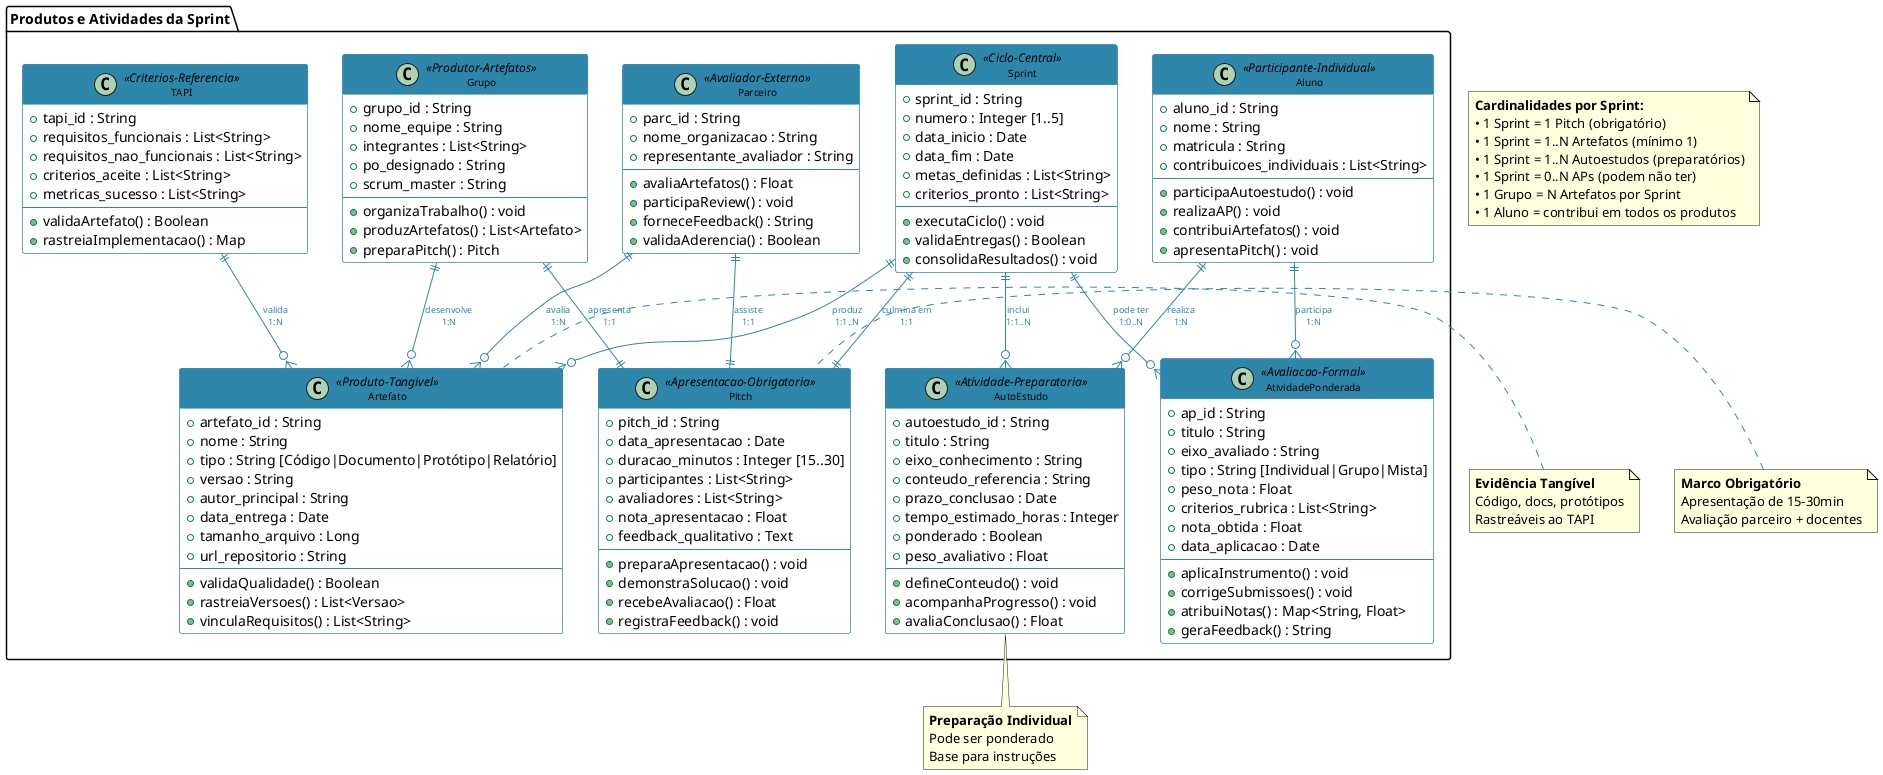
\includegraphics[width=0.9\textwidth]{plantuml/diagrama3_produtos_sprint}
    \caption{Produtos da Sprint: Artefatos, Pitch, Autoestudos e Atividades Ponderadas}
    \label{fig:produtos_sprint}
\end{figure}

Cada \textbf{Sprint} produz obrigatoriamente: 1..N \textbf{Artefatos}, exatamente 1 \textbf{Pitch}, 1..N \textbf{Autoestudos} e 0..N \textbf{Atividades Ponderadas}. \textbf{Grupos} desenvolvem Artefatos e apresentam Pitches, \textbf{Alunos} realizam Autoestudos e participam de APs. \textbf{Parceiro} avalia produtos conforme \textbf{TAPI}.

% ================================================================
% IDENTIFICADORES E RASTREABILIDADE
% ================================================================

\subsection{Identificadores Canônicos}

O modelo utiliza identificadores padronizados para rastreabilidade completa:

\begin{itemize}
    \item \textbf{dcn\_id} - Diretrizes Curriculares Nacionais
    \item \textbf{curso\_id} - Identificador do curso
    \item \textbf{metaproj\_id} - Identificador do metaprojeto
    \item \textbf{mod\_id} - Identificador do módulo
    \item \textbf{turma\_id} - Identificador da turma
    \item \textbf{grupo\_id} - Identificador do grupo
    \item \textbf{aluno\_id} - Identificador do aluno
    \item \textbf{sprint\_id} - Identificador da sprint
    \item \textbf{parc\_id} - Identificador do parceiro
    \item \textbf{tapi\_id} - Identificador do TAPI
    \item \textbf{artefato\_id} - Identificador do artefato
\end{itemize}

\textbf{Cadeia Hierárquica:} DCN → Curso → Metaprojeto → Módulo → Sprint → Artefato

\vspace{1em}
\hrule
\vspace{0.5em}
\textit{Arquivos fonte PlantUML atualizados: diagrama1\_modelo\_macro.puml, diagrama2\_estrutura\_operacional.puml, diagrama3\_produtos\_sprint.puml}